\documentclass[a4paper]{article}
\usepackage{fontspec}\defaultfontfeatures{Ligatures=TeX}
% \usepackage{setspace}\setstretch{1.3} % \begin{spacing}{1.3}
\usepackage[a4paper,vmargin={4cm,4cm},hmargin={4cm,4cm}]{geometry}
%-----------------------------------------------------------------------------%
\usepackage{settings}
%-----------------------------------------------------------------------------%
%%% Title %%%
\title{Von Neumann Ergodicity Theorem: An Introduction\thanks{This Introduction draws heavily from lecture note \cite{sarig-2023}.}}
\author{\href{https://jessekelighine.com}{jessekelighine.com}\\Jesse C.\ Chen\ 陳\,捷}
\date{\today}
%-----------------------------------------------------------------------------%
% [](https://joelmoreira.wordpress.com/2013/01/17/the-ergodic-theorem/)
% [](https://www.weizmann.ac.il/math/sarigo/sites/math.sarigo/files/uploads/ergodicnotes.pdf)
% [](http://math.uchicago.edu/~may/REU2017/REUPapers/Yunis.pdf)
% [](https://webspace.science.uu.nl/~kraai101/lecturenotes2009.pdf)

\begin{document}

\maketitle\thispagestyle{fancy}

\section{\glsentrylong{mps} and Ergodicity}

\begin{definition}[Measure Preserving System]
	A \emph{\gls{mps}} is a quadruple $(\Omega,\mathcal{B},\mu,\mathsf{T})$
	where $(\Omega,\mathcal{B},\mu)$ is a measure space, and
	\begin{enumerate}
		\item $\mathsf{T}:\Omega\to \Omega$ is a measurable transformation,
		\item $\mu$ is $\mathsf{T}$-invariance, i.e., $\mu(\mathsf{T}\inv E)=\mu(E)$ $\forall E\in\mathcal{B}$.
	\end{enumerate}
	If $\mu$ is a probability measure, then the quadruple is called a \gls{pps}.
\end{definition}

\begin{remark}
	The transformation $\mathsf{T}$ need not be rigid body motions when $\Omega=\reals^n$.
	Consider dividing up $\reals^n$ by grids into blocks and a transformation $\mathsf{T}$ that shuffles the blocks around.
	This is clearly a \gls{mps} when the space is equipped with Borel $\sigma$-algebra and Lebesgue measure.
\end{remark}

\begin{definition}[Ergodic]
	An \gls{pps} $(\Omega,\mathcal{B},\mu,\mathsf{T})$ is said to be \emph{ergodic}
	if $E\in\mathcal{B}$ is $\mathsf{T}$-invariant, i.e.,
	$E=\mathsf{T}\inv(E)$, then either $\mu(E)=0$ or $\mu(E)=1$.
\end{definition}

\begin{figure}[h]
	\centering
	\begin{subfigure}{0.4\textwidth}
		\centering
		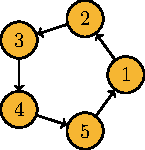
\includegraphics[scale=1]{figures/ergodic-mixing.pdf}
		\caption{Ergodic: well-mixed}
		\label{fig:ergodic}
	\end{subfigure}
	\begin{subfigure}{0.4\textwidth}
		\centering
		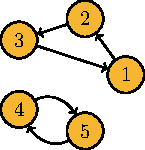
\includegraphics[scale=1]{figures/nonergodic-mixing.pdf}
		\caption{Non-ergodic: not well-mixed}
		\label{fig:nonergodic}
	\end{subfigure}
	\caption{Ergodic v.s.\ Non-ergodic \gls{pps}.}
	\label{fig:ergodic-vs-nonergodic}
\end{figure}

\begin{remark}
	An ergodic \gls{pps} is a system in which the only $\mathsf{T}$-invariant subspaces
	are either negligible (measure zero) or the entire space itself.
	That is, an ergodic \gls{pps} is a system that is ``well-mixed.''
	In \autoref{fig:ergodic-vs-nonergodic},
	two systems are shown
	where $\Omega=\{1,...,5\}$ and transformation $\mathsf{T}$ is denoted by arrows.
	In \autoref{fig:nonergodic}, there are two non-trivial $\mathsf{T}$-invariant subspaces that does not ``mix'' with each other;
	whereas in \autoref{fig:ergodic}, every element in $\Omega$ are ``mixed'' with each other.
\end{remark}

\begin{lemma}\label{lem:ergodic-characterization}
	Let $(\Omega,\mathcal{B},\mu,\mathsf{T})$ be an \gls{pps}, then the following are equivalent:
	\begin{enumerate}
		\item the \gls{pps} is ergodic,
		\item if $E\in\mathcal{B}$ and $\mu(E\triangle\mathsf{T}\inv E)=0$, then either $\mu(E)=0$ or $\mu(E)=1$,
		\item if $f:\Omega\to\reals$ is measurable and $f\circ\mathsf{T}=f$ a.e., then $f$ is constant a.e.
	\end{enumerate}
\end{lemma}
\begin{proof}
	We show (1.$\implies$2.), (2.$\implies$3.), and (3.$\implies$1.) respectively.
	\begin{itemize}
		\item(1.$\implies$2.)
			Suppose there is a set $E_0\in\mathcal{B}$ such that $E_0=\mathsf{T}\inv E_0$ and $\mu(E\triangle E_0)=0$.
			By ergodicity, we have $\mu(E_0)=0$ or $\mu(\Omega-E_0)=0$.
			And since $\mu(E\triangle E_0)=0$ implies $\mu(E)=\mu(E_0)$, we have $\mu(E)=0$ or $\mu(\Omega-E)=0$.

			Now we construct $E_0$.
			Consider the set $E_0=\{\omega\in\Omega:\mathsf{T}^{-k}(\omega)\in E\ \text{i.o.}\}$.
			Clearly, $E_0$ is measurable and $\mathsf{T}$-invariant.
			Also, we have $E\triangle E_0\subseteq\bigcup_{k\geq1}E\triangle\mathsf{T}^{-k}E$.
			Hence, we have
			\begin{align*}
				\mu(E\triangle E_0)
				&\leq \sum_{k\geq1} \mu(E\triangle\mathsf{T}^{-k}E) \\
				&\leq \sum_{k\geq1} \sum_{j=0}^{k-1} \mu(\mathsf{T}^{-j}E\triangle\mathsf{T}^{-(j+1)}E)
				= \sum_{k\geq1} k \mu(E\triangle \mathsf{T}\inv E)
			\end{align*}
			where the last inequality is obtained by the fact that
			\begin{align*}
				\mu(A_1\triangle A_2)\leq\mu(A_1\triangle A_3)+\mu(A_3\triangle A_2)
			\end{align*}
			for all $A_i\in\mathcal{B}$.
			Since $\mu(E\triangle \mathsf{T}\inv E)=0$, we have that $\mu(E\triangle E_0)=0$.
		\item(2.$\implies$3.)
			Let $f$ be a measurable function s.t.\ $f\circ\mathsf{T}=f$ a.e.
			For any $y\in\reals$, we have
			$[f>y]\triangle\mathsf{T}\inv[f>y]\subseteq[f\neq f\circ\mathsf{T}]$,
			hence
			\begin{align*}
				\mu([f>y]\triangle\mathsf{T}\inv[f>y]) = 0.
			\end{align*}
			By the assumption, either $\mu[f>y]=0$ or $\mu[f\leq y]=0$, i.e.,
			either $f>y$ a.e.\ or $f\leq y$ a.e.
			Let $c\coloneqq\sup\{y\in\reals:f>y\ \text{a.e.}\}$,
			then $f=c$ a.e.
		\item(3.$\implies$1.)
			Let $E\in\mathcal{B}$ satisfies $E=\mathsf{T}\inv(E)$.
			Consider $f=\one_{E}$.
			Since $f\circ\mathsf{T}=f$, $f$ is constant a.e.,
			we have $f=0$ a.e.\ or $f=1$ a.e.,
			implying that either $\mu(E)=0$ or $\mu(E)=1$.
			\qedhere
	\end{itemize}
\end{proof}

\begin{remark}
	The third characterization is quite interesting and intuitive.
	Consider again \autoref{fig:nonergodic},
	where the \gls{pps} is equipped with probability space $\Omega=\{1,...,5\}$, $\mathcal{B}=2^\Omega$, and uniform $\mu$.
	We can define the function $f$ as follows:
	\begin{align*}
		f(\omega) =
		\begin{cases}
			0 & \text{ if } \omega \in \{1,2,3\}, \\
			1 & \text{ otherwise.}
		\end{cases}
	\end{align*}
	It is clear that $f\circ\mathsf{T}=f$, but $f$ is not constant on $\Omega$.
	This is achievable since non-ergodicity means there are non-trivial $\mathsf{T}$-invariant subspaces,
	and we can simply define $f$ to be constant on each subspace.
	However, in \autoref{fig:ergodic}, since the system is ``well-mixed,''
	this trick is not possible.
\end{remark}

\begin{definition}[Strong Mixing]
	An \gls{pps} $(\Omega,\mathcal{B},\mu,\mathsf{T})$ is called \emph{strong mixing}
	if for any $E,F\in\mathcal{B}$ we have
	\begin{align*}
		\mu(E\cap\mathsf{T}\inv[n]F) \to \mu(E) \mu(F) \quad \text{ as } \quad n\to\infty.
	\end{align*}
\end{definition}

\begin{remark}
	The fact that strong mixing is defined using the inverse map of $\mathsf{T}$ is not merely due to measure-theoretic technicalities.
	The interpretation is ``no matter what obscure events $F$ one chooses,
	it could have been from all over in the system entirely randomly,
	not just some specific part.''
	Thus, for any other event $E$, the ``origins'' of $F$ must be as if independent of $E$.
\end{remark}

\begin{lemma}
	Strong mixing implies ergodicity.
\end{lemma}
\begin{proof}
	Suppose $(\Omega,\mathcal{B},\mu,\mathsf{T})$ is strong mixing.
	Let $E$ be such that $E=\mathsf{T}\inv E$, then we have
	\begin{align*}
		\mu(E) = \mu(E\cap\mathsf{T}\inv[n]E) \to \mu(E)^2 \quad \text{ as } \quad n\to\infty.
	\end{align*}
	Clearly, $\mu(E)=\mu(E)^2$ implies $\mu(E)$ is either $0$ or $1$.
\end{proof}

\section{Ergodicity Theorem}

\begin{theorem}[von Neumann's Ergodicity]\label{thm:von-neumann-ergodicity}
	Let $\mathcal{H}$ be a Hilbert space.
	Let $\mathsf{U}:\mathcal{H}\to \mathcal{H}$ be a unitary operator.
	Let $\mathcal{I}=\{f\in \mathcal{H}:\mathsf{U}f=f\}$ denote the $\mathsf{U}$-invariant subspace.
	Let $\mathsf{P}:\mathcal{H}\to\mathcal{I}$ be the orthogonal projection onto $\mathcal{I}$.
	Then, for any $f\in\mathcal{H}$, we have
	\begin{align}\label{eq:ergodicity}
		\frac1n \sum_{i=1}^{n} \mathsf{U}^i f
		\to
		\mathsf{P}f
		\quad\text{as}\quad
		n\to\infty
	\end{align}
	in the norm induced by the inner product on $\mathcal{H}$.
\end{theorem}
\begin{proof}
	Clearly, \autoref{eq:ergodicity} holds when $f\in\mathcal{I}$.
	Let $\mathcal{J}\coloneqq\{g-\mathsf{U}g:g\in\mathcal{H}\}$.
	Suppose $f\in\mathcal{J}$, we have
	\begin{align*}
		\innerprod{f,h}
		= \innerprod{g,h} - \innerprod{\mathsf{U}g,h}
		= \innerprod{g,h} - \innerprod{g,\mathsf{U}h}
		= 0 \quad \forall h\in\mathcal{I}.
	\end{align*}
	Hence, $\mathsf{P}f=0$.
	Furthermore, we have
	\begin{align*}
		\norm{ \frac1n \sum_{i=1}^{n} \mathsf{U}^{i}f }
		= \frac1n \norm{ \mathsf{U}g - \mathsf{U}^{n+1}g }
		\leq \frac1n \norm{ 2g }
		\to 0
		\quad\text{as}\quad
		n\to\infty.
	\end{align*}
	Therefore, \autoref{eq:ergodicity} holds for $\mathcal{J}$.

	We claim that \autoref{eq:ergodicity} also holds for the closure of $\mathcal{J}$,
	denoted by $\bar{\mathcal{J}}$.
	Suppose $f\in\bar{\mathcal{J}}$,
	then $\forall\varepsilon>0$ $\exists g\in\mathcal{J}$ s.t.\ $\norm{f-g}<\varepsilon$.
	Choose $N$ such that
	$\norm{ \frac1n \sum_{i=1}^{n} \mathsf{U}^{i}g } < \varepsilon$ $\forall n>N$.
	Then, we have
	\begin{align*}
		\norm{ \frac1n \sum_{i=1}^{n} \mathsf{U}^{i} f }
		\leq \norm{ \frac1n \sum_{i=1}^{n} \mathsf{U}^{i} (f-g) }
		+ \norm{ \frac1n \sum_{i=1}^{n} \mathsf{U}^{i} g } \leq 2\varepsilon.
	\end{align*}
	Thus, the claim holds.

	Lastly, we claim that $\bar{\mathcal{J}}^{\perp}=\mathcal{I}$.
	Suppose $f\perp\bar{\mathcal{J}}$, we have that $\forall g\in\mathcal{H}$,
	\begin{align*}
		0
		= \innerprod{f,g-\mathsf{U}g}
		= \innerprod{f,g} - \innerprod{f,\mathsf{U}g}
		\implies
		\innerprod{f,g}=\innerprod{\mathsf{U}^{*}f,g}.
	\end{align*}
	This implies that $f=\mathsf{U}f$ a.e., i.e., $f\in\mathcal{I}$.
	Conversely, we have shown that if $f\in\mathcal{J}$, then $f\perp\mathcal{I}$.
	Hence, the claim holds.
	And since $\mathcal{H}=\bar{\mathcal{J}}\oplus\mathcal{I}$,
	\autoref{eq:ergodicity} holds for all $f\in\mathcal{H}$.
\end{proof}

\begin{figure}[h]
	\centering
	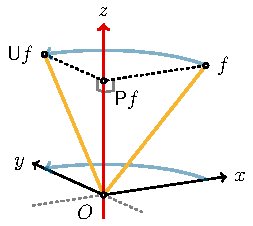
\includegraphics[scale=1]{figures/rotation.pdf}
	\caption{Visualization of \autoref{thm:von-neumann-ergodicity}.}
	\label{fig:ration}
\end{figure}

\begin{remark}
	If we think about \autoref{thm:von-neumann-ergodicity} in linear algebra terms,
	it lends itself to an intuitive understanding.
	In \autoref{fig:ration}, we consider $\reals^3$ space with $\mathsf{U}$ being a rotation along the $z$-axis.
	Clearly, a rotation is an unitary transformation,
	and its corresponding invariant subspace is exactly the $z$-axis.
	Consider an arbitrary vector $f$ and its transformations $\mathsf{U}^{i}f$.
	As $\mathsf{U}^{i}f$ rotates along the $z$-axis,
	it is clear that their ``average'' converges to $\mathsf{P}f$, the orthogonal projection of $f$ onto the $z$-axis.
	One can also easily see that vectors of the form $f-\mathsf{U}f$ is orthogonal to the $z$-axis.
\end{remark}

\begin{corollary}\label{cor:von-neumann-ergodicity}
	Let $(\Omega,\mathcal{B},\mu,\mathsf{T})$ be an \gls{pps}.
	If $f\in L^2(\Omega)$,
	then
	\begin{align*}
		\frac1n \sum_{i=1}^{n} f\circ \mathsf{T}^i
		\lto
		\bar{f}
		\quad\text{as}\quad
		n\to\infty
	\end{align*}
	where $\bar{f}\in L^2(\Omega)$ is $\mathsf{T}$-invariant.
	Furthermore, if $(\Omega,\mathcal{B},\mu,\mathsf{T})$ is ergodic, then
	\begin{align*}
		\bar{f}=\int_{\Omega}f\dd\mu.
	\end{align*}
\end{corollary}

\begin{proof}
	Note that $L^2(\Omega)$ is a Hilbert space.
	Let $\mathsf{U}f\coloneqq f\circ\mathsf{T}$.
	Since $\norm{f\circ\mathsf{T}}=\norm{f}$ for $f\in L^2(\Omega)$, $\mathsf{U}$ is unitary.
	Hence, the statement is a direct implication of \autoref{thm:von-neumann-ergodicity}.
	Furthermore, if the \gls{pps} is ergodic, then by \autoref{lem:ergodic-characterization},
	the $\mathsf{T}$-invariant subspace $\mathcal{I}$ contains only constant functions.
	Therefore, the orthogonal projection of $f$ onto $\mathcal{I}$ is its expectation.
\end{proof}
\begin{remark}
	The sum still converges without ergodicity, but this is not very useful, since we do not know the form of $\bar{f}$.
	With ergodicity, we know $\bar{f}$ is a constant function.
	Hence, we can simply pick any starting point $\omega\in\Omega$
	and compute $f\circ\mathsf{T}^{i}(\omega)$ along the way to obtain the same constant $\bar{f}$,
	without worrying about the entire functional space.
\end{remark}

\section{Markov Chains under the Language of Ergodicity}

Now we want to rephrase what we already understand about Markov chains under the language of von Neumann's Ergodicity Theorem.

\begin{definition}[\acrlong{sft}]
	Let $\mathcal{S}$ with be a finite set of states.
	Let $\mathsf{A}=(\mathsf{A}_{ij})_{\mathcal{S}\times\mathcal{S}}$
	be a adjacency matrix with $\mathsf{A}_{ij}\in\{0,1\}$ and without rows or columns be entirely zero.
	Let $\Omega_{\mathsf{A}}$ be defined as the space of possible sequences
	\begin{align*}
		\Omega_{\mathsf{A}} \coloneqq \{\omega=(\omega_0,\omega_1,...):\mathsf{A}_{\omega_i,\omega_{i+1}}=1\ \forall i\}.
	\end{align*}
	A \gls{sft} with states $\mathcal{S}$ with adjacency matrix $\mathsf{A}$ is the triple $(\Omega_{\mathsf{A}},d,\mathsf{T})$
	where $d(\omega,\omega')=2^{-\min\{k:\omega_k\neq\omega_k'\}}$ is a metric
	and $\mathsf{T}(\omega_0,\omega_1,...)=(\omega_1,\omega_2,...)$ is a shift transformation.
\end{definition}

\begin{remark}
	The topology generated by the metric $d(\cdot,\cdot)$ is equivalent to the topology generated by
	sets of the form
	\begin{align*}
		[s_0,...,s_{n-1}] \coloneqq \{\omega\in\Omega_{\mathsf{A}}:\omega_i=s_i\ \forall i\in\{0,...,n-1\}\}.
	\end{align*}
	This form are sometimes referred to as ``cylinders.''
	This is the product topology on $\mathcal{S}^{\naturals}$ when $\mathcal{S}$ is given the discrete topology.
\end{remark}

\begin{remark}
	The space $\Omega$ is simply all possible sequencing of $\mathcal{S}$ that is permitted by $\mathsf{A}$.
	Consider again \autoref{fig:ergodic-vs-nonergodic}, now with the arrows denoting the adjacency matrix $\mathsf{A}$,
	then \autoref{fig:ergodic} and \autoref{fig:nonergodic} generates different $\Omega_{\mathsf{A}}$'s.
	What we want next is a way to say ``how likely is any given sequence realized/observed.''
\end{remark}

\begin{definition}[Markov Measure]
	Given a transition matrix $\mathsf{P}$, i.e.,
	a matrix with each row consisting weights summing to one,
	and a probability vector $\pi$,
	we construct a measure $\mu$ by letting
	\begin{align*}
		\mu[s_0,...,s_{n-1}] \coloneqq \pi_{s_0} \mathsf{P}_{s_0s_1} \cdots \mathsf{P}_{s_{n-2}s_{n-1}}.
	\end{align*}
\end{definition}

\begin{remark}
	The definition of Markov measure extends to a unique probability measure on $\Omega_{\mathsf{A}}$
	with product topology via Carath\'eodory extension theorem.
\end{remark}

\begin{lemma}\label{lem:invariant-iff-stationary}
	$\mu$ is $\mathsf{T}$-invariant iff $\pi$ is stationary w.r.t.\ $\mathsf{P}$.
\end{lemma}
\begin{proof}
	Note that $\mu$ is $\mathsf{T}$-invariant iff $\mu[\cdot,\mathbf{s}]=\mu[\mathbf{s}]$ $\forall\mathbf{s}=(s_0,...,s_{n-1})$.
	That is,
	\begin{align*}
		\sum_{t\in\mathcal{S}} \pi_{t}\mathsf{P}_{t s_0}\mathsf{P}_{s_0s_1} \cdots \mathsf{P}_{s_{n-2}s_{n-1}}
		&= \pi_{s_0}\mathsf{P}_{s_0s_1} \cdots \mathsf{P}_{s_{n-2}s_{n-1}} \quad\forall\mathbf{s}\\
		\iff
		\sum_{t\in\mathcal{S}} \pi_{t}\mathsf{P}_{t s_0} &= \pi_{s_0} \quad\forall s_0\in\mathcal{S}.
		\qedhere
	\end{align*}
\end{proof}

\begin{remark}
	With \autoref{lem:invariant-iff-stationary}, we established that the system corresponding to the \gls{sft} is a measure preserving system
	as long as the Markov measure is constructed with a stationary distribution.
	It remains to ask the question: When is such system ergodic? When is such system strong mixing?
	From the intuition established previously, we know that...
	\begin{itemize}
		\item
			\emph{Ergodic} means that the system is ``well-mixed,''
			i.e., all the states should be able to be reached from any other state.
			This corresponds to the idea of \emph{irreducibility}.
		\item
			\emph{Strong mixing} means that the ``origin'' of any set could be all over the system entirely randomly,
			i.e., we shouldn't observe a set that follows some path.
			This corresponds to the idea of \emph{aperiodicity}.
	\end{itemize}
	It would turn out that our intuitions are spot on in describing what kinds of \gls{sft} are ergodic and strong mixing.
\end{remark}

\begin{definition}[Irreducible]
	A transition matrix $\mathsf{P}$ is called \emph{irreducible}
	if $\forall a,b\in\mathcal{S}$ $\exists s_1,...,s_{n-1}\in\mathcal{S}$ s.t.\ $\mathsf{P}_{a,s_1}\cdots\mathsf{P}_{s_{n-1},b}>0$.
	We denote this as $a\nto b$.
\end{definition}

\begin{lemma}\label{lem:gcd-independent}
	If $\mathsf{P}$ is irreducible, then $\gcd\{n\in\naturals:a\nto a\}$ is independent of $a$.
\end{lemma}
\begin{proof}
	Suppose $p_a=\gcd\{n:a\nto a\}$ and $p_b=\gcd\{n:b\nto b\}$ for $a,b\in\mathcal{S}$.
	Since $\mathsf{P}$ is irreducible,
	we have $a\nto[m_1]b\nto[m_b]b\nto[m_2]a$ for some $m_1,m_2\in\naturals$ and $m_b\in\{n:b\nto b\}$.
	Since $p_a\divides m_1+m_b+m_2$ and $p_b\divides m_b$, we must have $p_a\divides p_b$.
	Similarly, we have $p_b\divides p_a$ by swapping $a$ and $b$.
	Therefore, $p_a=p_b$.
\end{proof}

\begin{definition}[Period]\label{dfn:period}
	The \emph{period} of an $\mathsf{P}$ is $\gcd\{n:a\nto a\}$.
	An irreducible $\mathsf{P}$ is \emph{aperiodic} if $\gcd\{n:a\nto a\}=1$.
\end{definition}

\begin{remark}
	\autoref{dfn:period} is well-defined since
	\autoref{lem:gcd-independent} guarantees that as long as $\mathsf{P}$ is irreducible,
	then the period is independent of state.
\end{remark}

\begin{theorem}[Ergodicity for Markov Chains]\label{thm:ergodicity-for-markov-chains}
	Let $\mathsf{P}$ be a transition matrix and let $\mathsf{P}_{ab}^{n}$ denote the $(a,b)$-th element of $\mathsf{P}^n$.
	Let $\pi$ be a stationary distribution of $\mathsf{P}$.
	Then,
	\begin{enumerate}
		\item
			if $\mathsf{P}$ is irreducible, then as $n\to\infty$,
			\begin{align*}
				\frac1n \sum_{i=1}^{n} \mathsf{P}_{ab}^{n} \to \pi_{b} \quad\forall a,b\in\mathcal{S}.
			\end{align*}
		\item
			if $\mathsf{P}$ is irreducible and aperiodic, then as $n\to\infty$,
			\begin{align*}
				\mathsf{P}_{ab}^{n} \to \pi_{b} \quad\forall a,b\in\mathcal{S}.
			\end{align*}
	\end{enumerate}
\end{theorem}
\begin{proof}
	Omitted.
	See, e.g., Chapter 1.5 in \cite{sarig-2023} or Chapter 5.6 in \cite{durett-2019} for a proof.
\end{proof}

\begin{corollary}\label{cor:ireeducible-iff-ergodicity}
	Let $(\Omega_{\mathsf{A}},\mathcal{B},\mu,\mathsf{T})$ be the \gls{pps} corresponding to
	the \gls{sft} $(\Omega_{\mathsf{A}},d,\mathsf{T})$
	with Markov measure $\mu$ under transition matrix $\mathsf{P}$.
	If $\mathsf{P}$ is irreducible, then the \gls{pps} ergodic.
	Furthermore, if $\mathsf{P}$ is also aperiodic, then the \gls{pps} is strong mixing.
\end{corollary}
\begin{proof}
	First, note that
	for all cylinders $[\boldsymbol{a}]=[a_0,...,a_{n_a-1}]$ and $[\boldsymbol{b}]=[b_{0},...,b_{n_b-1}]$ and $k>n_a$,
	we have
	\begin{align}
		\mu([\boldsymbol{a}]\cap\mathsf{T}\inv[k][\boldsymbol{b}])
		&= \mu \left(\bigplus_{\boldsymbol{c}\in\mathcal{C}_{k-n_a}}[\boldsymbol{a},\boldsymbol{c},\boldsymbol{b}]\right) \nonumber\\
		&= \mu[\boldsymbol{a}]
		\left(
		\sum_{\boldsymbol{c}\in\mathcal{C}_{k-n_a}} \mathsf{P}_{a_{n_a-1},c_0}\cdots\mathsf{P}_{c_{k-n_a-1},b_0}
		\right)
		\frac{ \mu[\boldsymbol{b}] }{ \pi_{b_0} } \nonumber\\
		&= \mu[\boldsymbol{a}] \mu[\boldsymbol{b}] \frac{ \mathsf{P}_{a_{n_a-1},b_0}^{k-n_a} }{ \pi_{b_0} }
		\label{eq:cylinders-rearrange}
	\end{align}
	where $\mathcal{C}_{\ell} \coloneqq \{\boldsymbol{c}=(c_0,...,c_{\ell-1}):[\boldsymbol{a},\boldsymbol{c},\boldsymbol{b}]\neq\varnothing\}$.
	By \autoref{thm:ergodicity-for-markov-chains}, we have that
	\begin{align*}
		\frac1n \sum_{k=n_a+1}^{n} \mu([\boldsymbol{a}]\cap\mathsf{T}\inv[k][\boldsymbol{b}])
		= \mu[\boldsymbol{a}] \mu[\boldsymbol{b}] \frac1{\pi_{b_0}} \left( \frac1n\sum_{k=n_a+1}^{n} \mathsf{P}_{a_{n_a-1},b_0}^{k-n_a} \right)
		\to \mu[\boldsymbol{a}] \mu[\boldsymbol{b}].
	\end{align*}

	Now suppose that $\mathsf{P}$ is irreducible.
	Let $E\in\mathcal{B}$ be invariant,
	then $\exists[\boldsymbol{a}_1],...,[\boldsymbol{a}_m]$ s.t.\ $\mu(E\triangle\bigplus_{j=1}^{m}[\boldsymbol{a}_{j}])<\varepsilon$.
	Since the collection of cylinders forms a semi-algebra,
	such $[\boldsymbol{a}_1],...,[\boldsymbol{a}_m]$ always exists.
	Then,
	\begin{align*}
		\mu(E)
		= \mu(E\cap \mathsf{T}\inv[k]E)
		= \sum_{i=1}^{m} \sum_{j=1}^{m} \mu([\boldsymbol{a}_i]\cap \mathsf{T}\inv[k][\boldsymbol{a}_j]) \pm 2\varepsilon.
	\end{align*}
	Taking average over $k$, by the fact we mentioned above, we have
	\begin{align*}
		\mu(E)
		&=
		\sum_{i=1}^{m} \sum_{j=1}^{m}
		\left(
		\frac1n \sum_{k}^{n} \mu([\boldsymbol{a}_i]\cap \mathsf{T}\inv[k][\boldsymbol{a}_j])
		\right)
		\pm 2\varepsilon \nonumber\\
		&\to
		\sum_{i=1}^{m} \sum_{j=1}^{m}
		\mu[\boldsymbol{a}_i] \mu[\boldsymbol{a}_j] \pm 2\varepsilon
		= \left( \sum_{i=1}^{m} \mu[\boldsymbol{a}_j] \right)^2 \pm 2\varepsilon
		= (\mu(E)\pm\varepsilon)^2 \pm 2\varepsilon
	\end{align*}
	as $n\to\infty$.
	Therefore,
	take $\varepsilon\downarrow0$ and we have that $\mu(E)=\mu(E)^2$,
	which implies either $\mu(E)=0$ or $\mu(E)=1$.
	Hence, we have ergodicity.

	Now suppose further that $\mathsf{P}$ is aperiodic.
	By \autoref{thm:ergodicity-for-markov-chains} and \eqref{eq:cylinders-rearrange},
	we have
	$\mu([\boldsymbol{a}]\cap\mathsf{T}\inv[k][\boldsymbol{b}]) \to \mu[\boldsymbol{a}] \mu[\boldsymbol{b}]$
	as $k\to\infty$.
	By a similar argument with approximation using cylinders,
	we obtain the desired result.
\end{proof}

\begin{figure}[h]
	\centering
	\begin{subfigure}{0.4\textwidth}
		\centering
		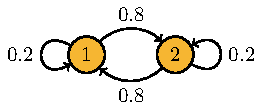
\includegraphics[scale=1]{figures/markov-periodic.pdf}
		\caption{Aperiodic}
		\label{fig:aperiodic}
	\end{subfigure}
	\begin{subfigure}{0.4\textwidth}
		\centering
		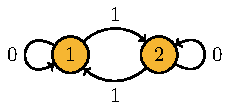
\includegraphics[scale=1]{figures/markov-aperiodic.pdf}
		\caption{Periodic}
		\label{fig:periodic}
	\end{subfigure}
	\caption{Markov Chains under different transition matrix $\mathsf{P}$.}
	\label{fig:markov-chains}
\end{figure}

\begin{remark}
	\autoref{fig:markov-chains} shows two Markov chains with same adjacency $\mathsf{A}$ but different transition $\mathsf{P}$.
	One can easily check both chains represented in \autoref{fig:aperiodic} and \autoref{fig:periodic}
	share the same invariant distribution $\pi=(0.5,0.5)$
	However, notice that \autoref{fig:periodic} has period $2$.
	% since if we are starting from state $1$, we must return to state $1$ on step $2$, set $4$, and so on.
	Hence, $\mathsf{P}_{11}^{n}$ converges to $0.5$ in \autoref{fig:aperiodic} but fails to converge in \autoref{fig:periodic}.
\end{remark}

\begin{remark}
	\autoref{cor:ireeducible-iff-ergodicity} can be extended to an if-and-only-if statement.
	The reverse statement can be proven using techniques similar to the proof of \autoref{cor:ireeducible-iff-ergodicity}.
\end{remark}

\printglossaries
\printbibliography

\end{document}
